\documentclass[a4paper 14pt]{article}
\usepackage{titlesec}
\setcounter{secnumdepth}{4}
\usepackage[utf8]{vietnam}
\usepackage{amsmath}
\usepackage{amsthm}
\usepackage{amsfonts}
\usepackage{amssymb}
\usepackage{float}
%\usepackage{multicolumns}

\usepackage[tmargin = 3cm, bmargin = 3.5cm, lmargin = 3.5cm, rmargin = 2cm]{geometry}
\usepackage{graphicx}
\graphicspath{{images/}}
\usepackage[belowskip = 5pt]{caption}
\captionsetup{
	font=footnotesize,
	justification=raggedright,
	singlelinecheck=false
}

%\setlength{\parskip}{1em}
%\setlength{\parindent}{4em}
\renewcommand{\baselinestretch}{1.5}
\begin{document}
	\begin{titlepage}
		\begin{center}
			%	\begin{tabular}{l}
			\large{\textbf{ĐẠI HỌC QUỐC GIA THÀNH PHỐ HỒ CHÍ MINH}}\\
			\large{\textbf{TRƯỜNG ĐẠI HỌC KHOA HỌC TỰ NHIÊN}}\\
			\large{\textbf{KHOA CÔNG NGHỆ THÔNG TIN}}\\
			%	\end{tabular}
			
			\vfill
			NGUYỄN PHAN MẠNH HÙNG - 1312727
			\vfill
			\Large{\textbf{ĐỒ ÁN MÔN HỌC }}\\
			\Large{DATAMINING}\\
		\end{center}
		\begin{flushleft}
			\vfill
			\large{\textbf{ĐỀ TÀI: KHAI THÁC CHUỖI PHỔ BIẾN}}\\
			\large{\textbf{DỰA TRÊN TÀI LIỆU: Sequential Pattern Mining using A Bitmap Representation. Authors: Jay Ayres, Johannes Gehrke, Tomi Yiu, and Jason Flannick}}
			\vfill
		\end{flushleft}
		\begin{center}
			TPHCM - 12/2015
		\end{center}
		
	\end{titlepage}
	\thispagestyle{empty}
	\tableofcontents
	\pagebreak
	\pagenumbering{arabic}
	\section*{Tóm tắt đồ án}
		Trong bài báo cáo này, người đọc sẽ trình bày các thuật toán để khai thác chuỗi phổ biến mà cụ thể là SPAM và SPADE. Bên cạnh đó, bài báo cáo cũng trình bày các cải tiến nhằm nâng cao hiệu quả của thuật toán bao gồm sử dụng BITMAP trong biểu diễn dữ liệu và tính toán độ hỗ trợ và sử dụng cấu trúc dữ liệu CMAP để giảm bớt các chuỗi không phổ biến xuất hiện trong quá trình duyệt dữ liệu.
	\section*{Tổng quan}
		Trong bài báo cáo sau đây, người viết sẽ trình bày các thuật toán SPAM và SPADE, kết hợp với cách biểu diễn dữ liệu theo dạng bitmap và sử dụng CMAP để tăng hiệu quả của thuật toán và giảm bớt không gian tìm kiếm.
	\section{Giới thiệu}
		Khai thác các chuỗi phổ biến là một trong những vấn đề vô cùng quan trọng trong khai thác dữ liệu. Việc rút trích được các chuỗi như vậy giúp chúng ta tìm ra được rất nhiều thông tin hữu ích có thể sử dụng để cải thiện hệ thống (hệ thống bán hàng, websites, hệ thống y sinh học...).
	\section{Phát biểu bài toán và các khái niệm liên quan}
		Gọi $I = \{i_1, i_2, \hdots, i_n\}$ là tập các item.
		Ta gọi tập con $X \subseteq I$ là một itemset.
		Một chuỗi $s = \langle s_1, s_2, \hdots, s_m \rangle$ là một danh sách các itemset có thứ tự. Trong đó $s_i \subseteq I$, và $i \in \{1,2,\hdots,m\}$.
		Độ dài $l$ của chuỗi $s = \langle s_1, s_2, \hdots, s_m \rangle$ được định nghĩa như sau:\\
		\begin{center}
		$l \overset{def}{=} \sum\limits_{i = 1}^{m}|s_i|$\\
		\end{center}
		Khi đó, một chuỗi với độ dài l sẽ được gọi là l-sequence. Một chuỗi $s_a = \langle a_1, a_2, \hdots, a_n \rangle$ được gọi là nằm trong chuỗi $s_b = \langle b_1, b_2, \hdots, b_m \rangle$, nếu tồn tại n số $1 \leq i_1 < i_2 < \hdots < i_n \leq m$, sao cho $a_1 \subseteq b_{i_1}, \hdots, a_2 \subseteq b_{i_2}$, khi đó chuỗi $s_a$ được xem là có thứ tự từ điển nhỏ hơn $s_b$ và kí hiệu là $s_a \leq s_b$ (lưu ý: nếu chuỗi $s_a$ không chứa $s_b$ và ngược lại thì không tồn tại quan hệ thứ tự giữa 2 chuỗi ấy).\\
		Một cơ sở dữ liệu D là một bộ ba gồm $(cid,tid,X)$. Trong đó $cid$ là chỉ số khách hàng (còn gọi là customer-id), $tid$ là chỉ số giao dịch (gọi là transaction-id) dựa vào thời điểm giao dịch, $X$ là itemset thỏa $X \subseteq I$. Ta cũng có thể biểu diễn cơ sở dữ liệu, trong đó mỗi khách hàng ứng với một chuỗi các itemset theo thứ tự thời gian (tid).\\
		\begin{table}[H]
			\begin{minipage}[t]{0.5\linewidth}
				\centering
				\begin{tabular}{|c | c | c|}
					\hline
					Customer ID & TID & Itemset\\ \hline
					1 & 1 & $\{a, b, d\}$\\ \hline
					1 & 3 & $\{b, c, d\}$\\ \hline
					1 & 6 & $\{b, c, d\}$\\ \hline
					2 & 2 & $\{b\}$\\ \hline
					2 & 4 & $\{a, b, c\}$\\ \hline
					3 & 5 & $\{a, b\}$\\ \hline
					3 & 7 & $\{b, c, d\}$\\ \hline
				\end{tabular}
				\caption{Cơ sở dữ liệu sắp xếp theo CID và TID}
				\label{table:type1}
			\end{minipage}%
			\begin{minipage}[t]{0.5\linewidth}
				\centering
				\begin{tabular}{| c | c |}
					\hline
					CID & Chuỗi\\ \hline
					1 & $\langle \{a, b, d\}, \{b, c, d\}, \{b, c, d\}\rangle$\\ \hline
					2 & $\langle \{b\}, \{a, b, c\} \rangle$\\ \hline
					3 & $\langle \{a, b\}, \{b, c, d\} \rangle$\\ \hline
				\end{tabular}
				\caption{Cơ sở dữ liệu theo từng khách hàng}
				\label{table:type2}
			\end{minipage}%
		\end{table}$~$\\
		Độ hỗ trơ tuyệt đối (absolute support) của một chuỗi $s_a$ là số lượng chuỗi trong cơ sở dữ liệu D (bảng \ref{table:type2}) chứa $s_a$. Độ hỗ trợ tương đối (relative support) là phần trăm chuỗi trong D chứa $s_a$. Độ hỗ trợ của chuỗi $s_a$ trong cơ sở dữ liệu D được kí hiệu $sup_D(s_a)$. Ví dụ, với $s_a = \langle \{a\}, \{b,c\} \rangle$. Dựa vào bảng 2, ta thấy chuỗi 1 và 3 chứa $s_a$, do đó $sup_D(s_a) = 2$.\\
		$~$\\
		\textbf{Đặt vấn đề:} Xét cơ sở dữ liệu D và minSup, hãy tìm tất cả các chuỗi thỏa minSup, nghĩa là với mỗi chuỗi s tìm được thì $sup_D(s) \geq minSup$.
		
	\section{Thuật toán SPAM - Sequential Pattern Mining}
		\subsection{Cây thứ tự - Lexicographic Tree}
			\begin{figure}[H]
				\includegraphics[scale = 0.9]{lextree}
				\caption{Ví dụ Lexicographic Tree}
			\end{figure}
			Ảnh trên mô tả một cây thứ tự thể hiện không gian các chuỗi tạo bởi các item cho trước. Mỗi nút n của cây sẽ tương ứng với một chuỗi, $s_c$  được tạo ra từ chuỗi cha, gọi là $s_p = \langle s_1, s_2, \hdots, s_k, \{a_1, a_2, \hdots, a_t\}\rangle$ thông qua S-step hoặc I-step.\\
			\begin{itemize}
				\item \textbf{S-step: $s_p \times item \overset{S-step}{\longrightarrow} s_c$}: $s_c = \langle s_1, s_2, \hdots, s_k, \{a_1, a_2, \hdots, a_t\}, \{item\}\rangle$ 
				\item \textbf{I-step: $s_p \times item \overset{I-step}{\longrightarrow} s_c$}: $s_c = \langle s_1, s_2, \hdots, s_k, \{a_1, a_2, \hdots, a_t, item\}\rangle$ 
			\end{itemize}
			Dựa vào định nghĩa trên, $s_p \leq s_c$ và với mọi nút n là cha, trực tiếp hay gián tiếp, của m thì $s_n \leq s_m$.\\
			Bên cạnh đó, với tập item hữu hạn bao gồm tất cả item trong database và gọi N là độ dài tối đa của chuỗi xuất hiện trong database, ta có thể sinh ra 1 cây hữu hạn nút thỏa mãn với mọi chuỗi trong database đều tồn tại một nút trong cây chứa chuỗi đó.
		\subsection{Tỉa nhánh cây - Pruning}
			Bây giờ, bài toán của ta trở thành tìm các chuỗi phổ biến trên cây. Tuy vậy, ta thấy kích thước của cây (số nút) là khá lớn, do đó cần phải có một chiến lược tỉa nhánh hợp lý nhằm thu hẹp không gian tìm kiếm.\\
			Để thuận tiện, ta định nghĩa $S_n$ là tập các item dùng trong S-step với nút n, và $I_n$ là tập các item dùng trong I-step với n.
			\subsubsection{S-step pruning}
				Xét chuỗi s và 2 chuỗi $s_a = \langle s, {i_k} \rangle$ và $s_b = \langle s, {i_j} \rangle$ được sinh từ s thông qua S-step. Giả sử $i_k \leq i_j$, $s_a$ là chuỗi phổ biến và $s_b$ không phổ biến. Theo nguyên tắc Apriori thì chuỗi $s_c = \langle s, \{i_k, i_j\}\rangle$ và chuỗi $s_d = \langle s, \{i_k\}, \{i_j\}\rangle$ đều không phổ biến. Do đó, ta có thể loại item $i_j$ ra khỏi $S_g$ và $I_g$, với $s_g$ là tất cả các chuỗi phổ biến được sinh ra từ s qua S-step.
			\subsubsection{I-step pruning}
				Xét chuỗi $s = \langle s', \{i_1, \hdots, i_t\}\rangle$ và 2 chuỗi $s_a = \langle s', \{i_1, \hdots, i_t, i_k\} \rangle$ và $s_a = \langle s', \{i_1, \hdots, i_t, i_j\} \rangle$ được sinh từ s thông qua I-step. Giả sử $i_k \leq i_j$, $s_a$ là chuỗi phổ biến và $s_b$ không phổ biến. Theo nguyên tắc Apriori thì chuỗi $s_c = \langle s', \{i_1, \hdots, i_t, i_k, i_j\}\rangle$ không phổ biến. Do đó, ta có thể loại item $i_j$ ra khỏi $I_g$, với $s_g$ là tất cả các chuỗi phổ biến được sinh ra từ s qua I-step.
		\subsection{Biểu diễn cơ sở dữ liệu và chuỗi bằng Bitmap và các phép toán trên Bitmap}
			Ta có nhận xét rằng chi phí cho việc tính độ hỗ trợ của 1 chuỗi là khá lớn vì ta phải liên tục duyệt lại cơ sở dữ liệu. Do đó, ta cần phải biểu diễn dữ liệu bằng một cấu trúc hiệu quả hơn.
			\subsubsection{Cách biểu diễn}
				Với mỗi item, ta sẽ tạo 1 bitmap tương ứng trong đó mỗi bit tương ứng với một transaction. Để thuận tiện, các transaction trong cùng một sequence (của một customer) sẽ được biểu diễn bằng các bits gần nhau. Và để đảm bảo tính thứ tự, nếu transaction m đứng trước transaction n trong sequence thì chỉ số bit biểu diễn m sẽ nhỏ hơn chỉ số của bit biễu diễn n. Ví dụ, bitmap biểu diễn item a trong dữ liệu mẫu được thể hiện như sau: \\
				\begin{table}[H]
					\begin{minipage}[t]{0.4\linewidth}
						\begin{tabular}{|c | c | c |}
							\hline
							CID & TID & $\{a\}$\\
							\hline
							1 & 1 & 1 \\
							1 & 3 & 0 \\
							1 & 6 & 0 \\
							- & - & 0 \\
							\hline
							2 & 2 & 0 \\
							2 & 4 & 1 \\
							- & - & 0 \\
							- & - & 0 \\
							\hline
							3 & 5 & 1 \\
							3 & 7 & 0 \\
							- & - & 0 \\
							- & - & 0 \\
							\hline
						\end{tabular}
						\caption{Bitmap biểu diễn item a}
					\end{minipage}
				\end{table}
				Bên cạnh đó, ta xây dựng bitmap cho một chuỗi như sau: nếu itemset cuối cùng của chuỗi nằm trong transaction j của khách hàng a và tất cả các itemset khác nằm ở transaction trước j, thì bit biểu diễn transaction j của khách a được gán 1, ngược lại là 0. Ví dụ, chuỗi $\langle \{a\}, \{b\} \rangle$\\
					\begin{table}[H]
						\begin{minipage}[t]{0.5\linewidth}
							\begin{tabular}{| c | c | c |}
								\hline
								CID & TID & $\langle \{a\}, \{b\} \rangle$\\
								\hline
								1 & 1 & 0 \\
								1 & 3 & 1 \\
								1 & 6 & 1 \\
								- & - & 0 \\
								\hline
								2 & 2 & 0 \\
								2 & 4 & 0 \\
								- & - & 0 \\
								- & - & 0 \\
								\hline
								3 & 5 & 0 \\
								3 & 7 & 1 \\
								- & - & 0 \\
								- & - & 0 \\
								\hline
							\end{tabular}
							\caption{Bitmap biểu diễn chuỗi $\langle \{a\}, \{b\} \rangle$}
						\end{minipage}
					\end{table}
				Ta gọi mỗi phần được chia ra bởi đường ngang trên là một phân đoạn, thể hiện chuỗi đang xét có xuất hiện trong sequence của khách hàng tương ứng không. Với cách biểu diễn trên, để tính độ hỗ trợ của một chuỗi, ta chỉ cần kiểm tra số lượng phân đoạn có ít nhất một bit 1. Ở ví dụ trên thì support($\langle \{a\}, \{b\} \rangle$) = 2, do phân đoạn ứng với CID bằng 1 và 3 có bit 1 xuất hiện. 
			\subsubsection{Các phép toán}
				Xét chuỗi $s = \langle \{a\} \rangle$, item b. Gọi Bitmap(s) là bitmap thể hiện chuỗi s.\\
				\begin{itemize}
					\item \textbf{S-step:} Gọi t là chuỗi được sinh từ s và item b thông qua S-step. Khi đó, Bitmap(t) = Pbitmap(s) and Bitmap(item b). Trong đó Pbitmap(s) được xây dựng từ Bitmap(s) (ta gọi bước biến đổi này là S-step process), có số lượng bit cũng như phân đoạn tương ứng, như sau: xét một phân đoạn của Bitmap(s), gọi k là vị trí bit 1 đầu tiên của phân đoạn. Khi đó các bit từ đầu phân đoạn tới k của Pbitmap(s) được gán 0, các bit còn lại gán 1. Ta làm tương tự với các phân đoạn khác của Pbitmap(s). 
					\item \textbf{I-step:} Gọi t là chuỗi được sinh từ s và item b thông qua I-step. Khi đó Bitmap(t) = Bitmap(s) and Bitmap(item b).
				\end{itemize}
				Ví dụ:
				\begin{figure}[H]
					\begin{minipage}[t]{0.5\linewidth}
						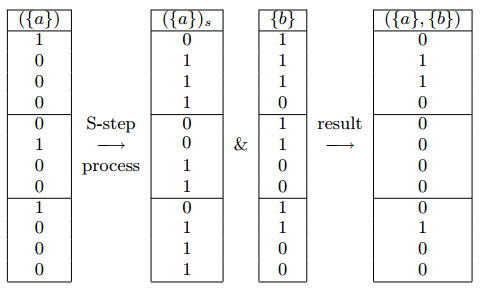
\includegraphics[scale = 0.5]{Sstep}
						\caption{S-step}
					\end{minipage}%
					\begin{minipage}[t]{0.5\linewidth}
						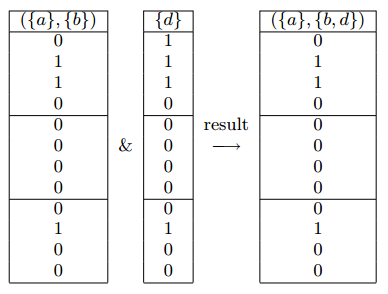
\includegraphics[scale = 0.5]{Istep}
						\caption{I-step}
					\end{minipage}%
				\end{figure}
		\subsection{Mã nguồn}
			\includegraphics[scale = 0.6]{spam}
		\subsection{Ví dụ}
			Xét lại cơ sở dữ liệu được đề cập trong bảng \ref{table:type2}\\
			Xét trường hợp gọi DFS với $n = \langle \{a\} \rangle,~S_n = \{a,b,c,d\},~I_n=\{b,c,d\}$\\
			DFS:
			\begin{enumerate}
				\item $S_{temp} = \emptyset, I_{temp} = \emptyset$
				\item Với mỗi $i \in S_n$, xét chuỗi $\langle \{a\}, \{i\} \rangle$\\
					\begin{tabular}{|c|c|}
						\hline
						S-sequence & Support \\ \hline
						$\langle \{a\}, \{a\} \rangle$ & 0 (không phổ biến) \\ \hline
						$\langle \{a\}, \{b\} \rangle$ & 2 \\ \hline
						$\langle \{a\}, \{c\} \rangle$ & 2 \\ \hline
						$\langle \{a\}, \{d\} \rangle$ & 2 \\ \hline
					\end{tabular}\\
					$\Rightarrow S_{temp} = \{b,c,d\}$
					Gọi DFS với\\
					\begin{enumerate}
						\item $n = \langle \{a\} \{b\} \rangle,~S_n = \{b,c,d\},~I_n=\{c,d\}$
						\item $n = \langle \{a\} \{c\} \rangle,~S_n = \{b,c,d\},~I_n=\{d\}$
						\item $n = \langle \{a\} \{d\} \rangle,~S_n = \{b,c,d\},~I_n=\emptyset$
					\end{enumerate}
				\item Với mỗi $i \in I_n$, xét chuỗi $\langle \{a,i\} \rangle$\\
					\begin{tabular}{|c|c|}
						\hline
						S-sequence & Support \\ \hline
						$\langle \{a,b\} \rangle$ & 3  \\ \hline
						$\langle \{a,c\} \rangle$ & 1 (không phổ biến)\\ \hline
						$\langle \{a,d\} \rangle$ & 1 (không phổ biến)\\ \hline
					\end{tabular}\\
					$\Rightarrow I_{temp} = \{b\}$\\
					Gọi DFS với
					\begin{enumerate}
						\item $n = \langle \{a,b\} \rangle,~S_n = \{b,c,d\},~I_n=\emptyset$
					\end{enumerate}
			\end{enumerate}
			
	\section{Thuật toán SPADE}
		\subsection{Khái niệm cơ bản}
			Ở đây, ta thu hẹp định nghĩa sequence lại. Lúc này mỗi itemset trong sequence chỉ chứa duy nhất một item.\\
			Gọi $F_k$ là tập tương đương kích thước k. Các phần tử của $F_k$ bao gồm các chuỗi có độ dài k và có chung prefix là k-1 item đầu. Bên cạnh đó, ta giữ nguyên cái khái niệm, định nghĩa về bitmap, s-step, và i-step như trong phần vừa trình bày.
		\subsection{Phương pháp}
			Trình tự thực hiện thuật toán.
			\begin{enumerate}
				\item Đầu tiên, ta sinh tập $F_1$ gồm các chuỗi phổ biến (giả sử $F_1$ có k phần tử). Gọi Enumerate($F_1$).
				\item\label{start} Với mỗi chuỗi $A_i$ thuộc F, ta khởi tạo $T_i$ rỗng. 
				\item Sau đó với mỗi $j \geq i$, ta sinh chuỗi $r = Merge(A_i, A_j)$. Nếu r phổ biến thì $T_i = T_i \cup \{r\}$
				\item Gọi Enumerate($T_i$)
				\item Nếu $i \leq |F|$, quay lại bước \ref{start}
			\end{enumerate}  
			Giải thích hàm $Merge(A_i, A_j)$: gọi u, v lần lượt là item cuối cùng của $A_i$ và $A_j$. Giả sử u xuất hiện trong giao dịch trước giao dịch chứa v trong chuỗi dữ liệu. Khi đó, chuỗi r được sinh bằng cách thực hiện S-step trên chuỗi $A_i$ và item v.\\
			Bên cạnh đó, ta cũng có thể sử dụng Bitmap để tăng tốc cho thuật toán này.
		\subsection{Mã nguồn}
			\includegraphics[scale = 0.5]{spade} 
		\subsection{Ví dụ}
			Xét cơ sở dữ liệu:\\
			\begin{tabular}{|c | c |}
				\hline
				ID & Sequence\\ \hline
				$s_1$ & CAAGAAGT\\ \hline
				$s_2$ & TGACAG\\ \hline
				$s_3$ & GAAGT\\ \hline
			\end{tabular}\\
			Tạo cơ sở dữ liệu theo chiều dọc:
			\begin{table}[H]
				\begin{minipage}[t]{0.2\linewidth}
					\begin{tabular}{|c|c|}
						\hline
						\multicolumn{2}{|c|}{A} \\ \hline
						1 & 2, 4, 5\\ \hline
						2 & 3, 5\\ \hline
						3 & 2, 3\\ \hline
					\end{tabular}
				\end{minipage}%
				\begin{minipage}[t]{0.2\linewidth}
					\begin{tabular}{|c|c|}
						\hline
						\multicolumn{2}{|c|}{C} \\ \hline
						1 & 1\\ \hline
						2 & 4\\ \hline
					\end{tabular}
				\end{minipage}%
				\begin{minipage}[t]{0.2\linewidth}
					\begin{tabular}{|c|c|}
						\hline
						\multicolumn{2}{|c|}{G} \\ \hline
						1 & 3, 6\\ \hline
						2 & 2, 6\\ \hline
						3 & 1, 4\\ \hline
					\end{tabular}
				\end{minipage}%
				\begin{minipage}[t]{0.2\linewidth}
					\begin{tabular}{|c|c|}
						\hline
						\multicolumn{2}{|c|}{T} \\ \hline
						1 & 7\\ \hline
						2 & 1\\ \hline
						3 & 5\\ \hline
					\end{tabular}
				\end{minipage}%
			\end{table}
			$\Rightarrow F_1 = \{A, G, T\}$, do C không phổ biến.\\
			Enumerate(F1):
			\begin{enumerate}
				\item Xét $A_1 = A \in F$ \label{startloop}
					\begin{enumerate}
							\item $T_1 = \emptyset$
							\item Với mỗi $A_j \in F$, mà $j \geq i = 1$, thì $R = A_i \cup A_j$\\ 
							\begin{tabular}{|c|c|c|}
								\hline
								$A_j$ & R & support(R) \\ \hline
								A & AA & 3\\ \hline
								G & AG & 3\\ \hline
								T & AT & 2 (không phổ biến)\\ \hline
							\end{tabular}\\
							$\Rightarrow T_1 = \{AA, AG\}$
					\end{enumerate}
				\item Enumerate($T_1$)
				\item Quay lại bước \ref{startloop} cho tới khi duyệt hết tập F.
			\end{enumerate}
			
			
	\section{Ứng dụng CMAP để loại bỏ chuỗi không phổ biến}
		Trong phần này, ta sẽ dùng cơ sở dữ liệu sau để trình bày
		\begin{table}[H]
			\begin{tabular}{| c | c |}
				\hline
				SID & Chuỗi\\ \hline
				1 & $\langle \{a,b\}, \{c\}, \{f,g\}, \{g\}, \{e\} \rangle$\\ \hline
				2 & $\langle \{a,d\}, \{c\}, \{b\}, \{a,b,e,f\} \rangle$\\ \hline
				3 & $\langle \{a\}, \{b\}, \{f\}, \{e\} \rangle$\\ \hline
				4 & $\langle \{b\}, \{f,g\}\rangle$\\ \hline
			\end{tabular}
		\end{table}
		\subsection{Định nghĩa}
			CMAP là một cấu trúc dữ liệu ánh xạ mỗi item thành một tập các item nằm sau nó.Gồm 2 loại:
			\begin{enumerate}
				\item $CMAP_i$
				\item $CMAP_s$
			\end{enumerate}
			\subsubsection{$CMAP_i$}
				Một item y thuộc $CMAP_i(x)$ khi và chỉ khi chuỗi $\langle \{x,y\} \rangle$ phổ biến. Ví dụ:
				\begin{table}[H]
						\begin{tabular}{| c | c |}
						\hline
						\multicolumn{2}{|c|}{$CMAP_i$}\\ \hline
						item & $CMAP_i(item)$\\ \hline
						a & \{b\} \\ \hline
						b & $\emptyset$ \\ \hline
						c & $\emptyset$ \\ \hline
						e & $\emptyset$ \\ \hline
						f & \{g\} \\ \hline
						g & $\emptyset$ \\ \hline
						\end{tabular}
				\end{table}
			\subsubsection{$CMAP_s$}
				Một item y thuộc $CMAP_s(x)$ khi và chỉ khi chuỗi $\langle \{x\}, \{y\} \rangle$ phổ biến. Ví dụ:
				\begin{table}[H]
					\begin{tabular}{| c | c |}
						\hline
						\multicolumn{2}{|c|}{$CMAP_i$}\\ \hline
						item & $CMAP_i(item)$\\ \hline
						a & \{b,c,e,f\} \\ \hline
						b & \{e,f,g\} \\ \hline
						c & \{e,f\} \\ \hline
						e & $\emptyset$ \\ \hline
						f & \{e,g\} \\ \hline
						g & $\emptyset$ \\ \hline
					\end{tabular}
				\end{table}
		\subsection{Ứng dụng CMAP}
			Xét chuỗi $\langle s_1, s_2, \hdots, \{i_1, i_2, \hdots, i_t\} \rangle$ và item k. Ta sử dụng 2 nhận xét sau:
			\begin{itemize}
				\item Nếu $k \notin CMAP_i(i_1) \cap CMAP_i(i_2) \cap \hdots \cap CMAP_i(i_t)$, thì chuỗi $\langle s_1, s_2, \hdots, \{i_1, i_2, \hdots, i_t, k\}\rangle$ không phổ biến.
				\item Nếu $\exists j \in s, \text{ mà } k \notin CMAP_s(j)$ thì $\langle s_1, s_2, \hdots, \{i_1, i_2, \hdots, i_t\}, \{k\} \rangle$ không phổ biến.
			\end{itemize}
			Áp dụng nhận xét trên vào các thuật toán SPAM và SPADE, ta có thể loại bỏ chuỗi được sinh ra để nhằm giảm bớt chi phí tính toán độ hỗ trợ.\\
			Ví dụ:
			\begin{itemize}
				\item Xét dãy $s = \langle \{a\}, \{f\} \rangle$\\
				Ta thấy $CMAP_I(f) = \{g\}$, do đó ta có thể mở rộng chuỗi s thông qua I-step với item g.
				\item Xét dãy $s = \langle \{a\}, \{c\} \rangle$.\\
				Ta thấy $CMAP_S(a) \cap CMAP_S(c) = \{b,c,e,f\} \cap \{e,f\} = \{e,f\}$, do đó ta có thể mở rộng chuỗi s thông qua S-step với item thuộc tập $\{e,f\}$
			\end{itemize}
		\subsection{Biểu diễn CMAP}
			Ta có thể biểu diễn CMAP một cách dễ dàng bằng mảng 2 chiều kiểu BOOL, trong đó dòng phần tử (i,j) mang giá trị TRUE nếu item j nằm trong CMAP(i) và FALSE nếu không. Tuy vậy, trong thực tế thì ta thấy rằng kích thước CMAP khá nhỏ, do đó để tiết kiệm bộ nhớ ta thường sử dụng bảng băm để lưu trữ cặp (i,j) mang giá trị TRUE. Điều này sẽ giảm đáng kể dữ liệu được sử dụng.
	\section{Đánh giá thực nghiệm}
		Ta sử dụng các cơ sở dữ liệu sau để đánh giá.\\
		\begin{figure}[H]
			\includegraphics[scale = 0.5]{datafeature}
			\caption{Bảng mô tả cơ sở dữ liệu trong thực nghiệm}
		\end{figure}
		
		\begin{figure}[H]
			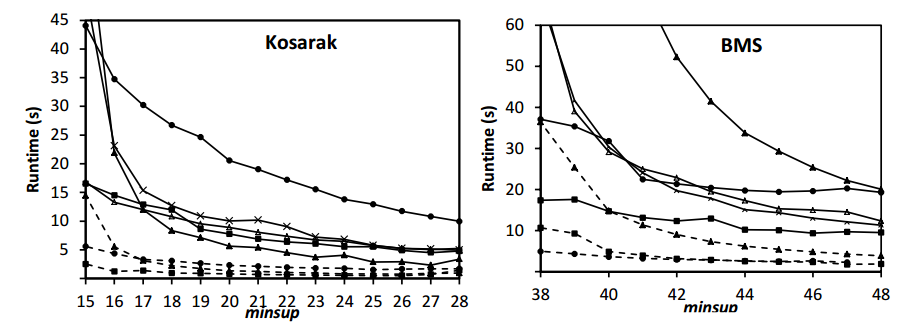
\includegraphics[scale = 0.5]{BMS_KOSARAK}
			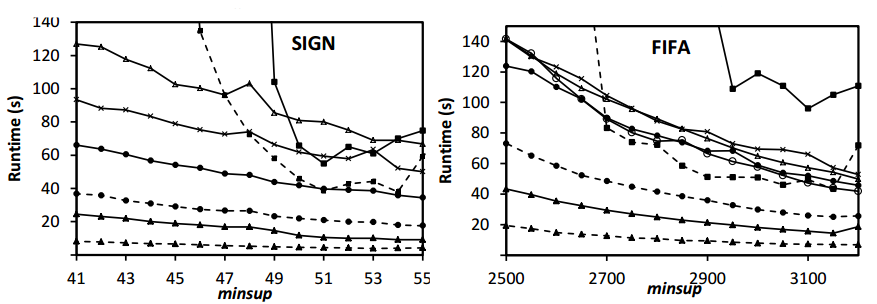
\includegraphics[scale = 0.5]{FIFA_SIGN}
			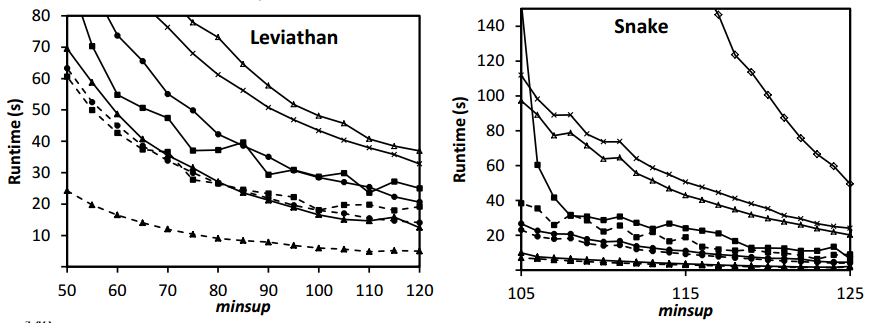
\includegraphics[scale = 0.5]{SNAKE_LEVI}
			\includegraphics[scale = 0.5]{Legend}
		\end{figure}
		
	\section{Kết luận}
		Thông thường, các thuật toán khai thác chuỗi phổ biến sử dụng cấu trúc dữ liệu theo chiều dọc (vertical database) thường rất hiệu quả vì chúng có thể tính toán độ hỗ trợ rất tốt do tránh phải duyệt cơ sở dữ liệu (thường rất lớn) nhiều lần. Tuy vậy, các thuật toán này cũng gặp phải khó khăn do phải duyệt các chuỗi thường không tồn tại trong cơ sở dữ liệu. Để giảm bớt điều đó, ta có thể kết hợp cấu trúc dữ liệu CMAP đã được đề cập để giảm bớt các chuỗi không cần thiết.
	%\section{Tham khảo}
	\begin{thebibliography}{9}
		
		\bibitem{SPAM}
		Jay Ayres, Johannes Gehrke, Tomi Yiu, and Jason Flannick. \emph{Sequential PAttern Mining using A Bitmap Representation}
		\bibitem{SPADE} Philippe Fournier-Viger, Antonio Gomariz, Manuel Campos, and Rincy Thomas. \emph{Fast Vertical Mining of Sequential Patterns Using Co-occurrence Information}
		\bibitem{SPADE} Mohammed J. Zaki, Wagner Meira Jr. . \emph{DATA MINING AND ANALYSIS Fundamental Concepts and Algorithms,} $1^{st}$ edition, Cambridge University Press, New York, 2014.
	\end{thebibliography}
\end{document}